\documentclass[12pt]{article}
\usepackage{amsmath}
\usepackage{tikz}
\begin{document}
\title{Computer Science M151B, Homework 7}
\date{May 21st, 2018}
\author{Michael Wu\\UID: 404751542}
\maketitle

\section*{Problem 1}

For the transfer using 4-word blocks, each transfer will take 1 cycle to send the address to memory, 24 cycles to access memory for the first
set of words, 1 cycle to send the data from memory, and 2 idle clock cycles. So each 4-word block takes 28 cycles to read. This is 140 ns for each
4-word block. Thus the sustained bandwidth of the read is
\[4\,\frac{\text{words}}{\text{block}}\times 4\,\frac{\text{bytes}}{\text{word}}\times \frac{1 \text{ block}}{1.4 \times 10^{-7} \text{ s}}
=1.1423 \times 10^8\,\frac{\text{bytes}}{\text{s}}\]
The latency to transfer 256 words is then
\[\frac{256 \text{ words}}{4\,\frac{\text{words}}{\text{block}}}\times 140\,\frac{\text{ns}}{\text{block}}=8960 \text{ ns}\]
and the number of bus transactions per second is
\[\frac{1 \text{ transaction}}{1.4 \times 10^{-7} \text{ s}}=7.143 \times 10^{6}\,\frac{\text{transactions}}{\text{s}}\]

For the transfer using 16-word blocks, each transfer will take 1 cycle to send the address to memory, 24 cycles to access memory for the first
set of words, 1 cycle for each 4-word block to send the data from memory, and 2 idle clock cycles for each 4-word block. So each 16-word block
takes 37 cycles to read. This is 185 ns for each
16-word block. Thus the sustained bandwidth of the read is
\[16\,\frac{\text{words}}{\text{block}}\times 4\,\frac{\text{bytes}}{\text{word}}\times \frac{1 \text{ block}}{1.85 \times 10^{-7} \text{ s}}
=3.4595 \times 10^8\,\frac{\text{bytes}}{\text{s}}\]
The latency to transfer 256 words is then
\[\frac{256 \text{ words}}{16\,\frac{\text{words}}{\text{block}}}\times 185\,\frac{\text{ns}}{\text{block}}=2960 \text{ ns}\]
and the number of bus transactions per second is
\[\frac{1 \text{ transaction}}{1.85 \times 10^{-7} \text{ s}}=5.405 \times 10^{6}\,\frac{\text{transactions}}{\text{s}}\]

\section*{Problem 2}

In DMA-based I/O, an interrupt must still be given to the CPU to indicate that the device controller has finished an I/O request and put some data in memory.
The difference between interrupt-driven I/O and DMA-based I/O is that the interrupt-driven I/O will send an interrupt for every piece of data. The data in
interrupt-driven I/O always passes through the CPU prior to going to memory, whereas in DMA-based I/O the device controller can directly modify memory.
Thus DMA-based I/O introduces complexity into a computer's design because it may cause cache coherency problems. If the device controller modifies data in memory
that has changed somewhere higher in the cache, the CPU may accidentally use the wrong data which would lead to incorrect behaviour.

Interrupt-driven I/O would be preferred for simpler devices where the performance penalty is small compared to DMA-based I/O. If a lot of data is not being transferred
to memory at a time, then the advantage of DMA-based I/O being able to pass data quickly to memory is diminished. For example, if there is a sensor that generates one byte
every second and sends it to the processor, then interrupt-driven I/O would be preferred. This is because the device does not use a lot of CPU time, so the performance improvement
of DMA-based I/O would not be significant. If DMA-based I/O were used, this would add unnecessary complexity.

\pagebreak

\section*{Problem 3}

\begin{figure}[!ht]
        \vspace*{-1.5cm}
        \begin{center}
                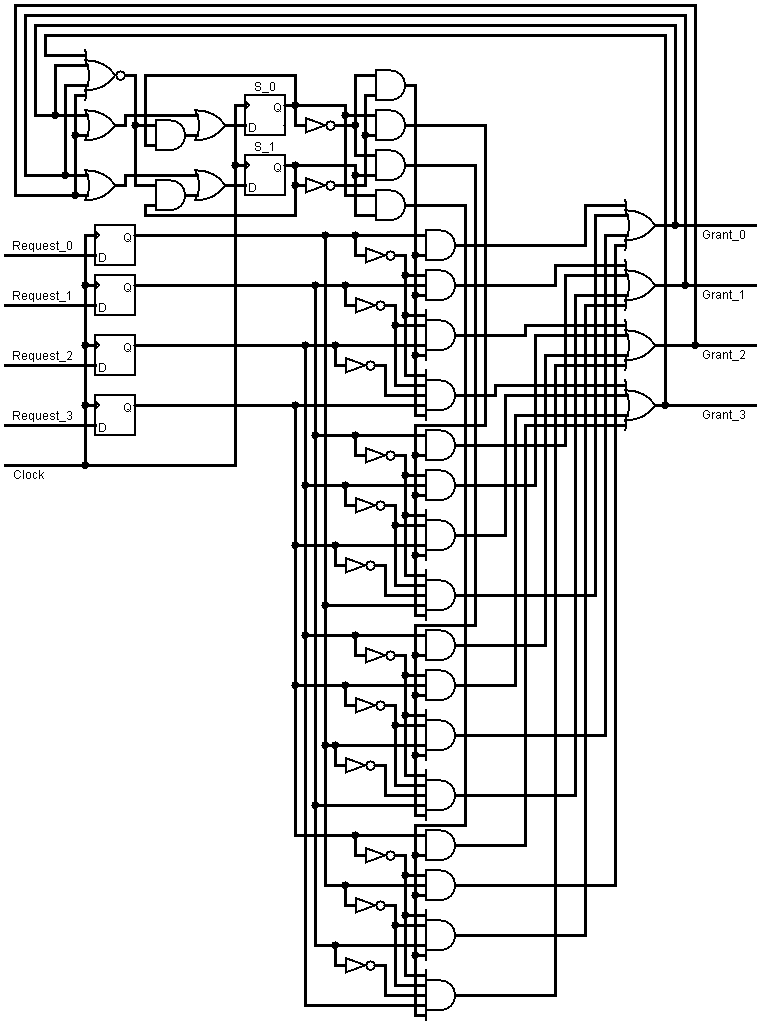
\includegraphics[width=5.4in]{problem3a.png}
        \end{center}
        \vspace*{-4cm}
\end{figure}

\clearpage

\paragraph{a)}

My arbiter design is shown above. It uses D flip-flops to keep track of a state variable \(S\) which indicates which device has the highest priority. This
signal gets decoded into four signals, each of which enables four of the sixteen \texttt{and} gates that control which grant line the arbiter will assert. I \texttt{or}
together the outputs of the \texttt{and} gates that correspond to a grant for a particular device in order to get the output grant signals. Finally,
if a grant is given then the state variable is updated to the next highest priority device. If no grant is given, the \texttt{nor} gate ensures that
the state stays at the same value. I also use D flip-flops on the input request lines to ensure that the grant stays asserted for a whole cycle. The logic that this design implements is shown below.

\[
        \begin{array}{c|c|c|c|c|c||c|c|c|c|c|c}
                \multicolumn{6}{c||}{\text{Inputs}} & \multicolumn{6}{|c}{\text{Outputs}}\\
                \hline
                R_0 & R_1 & R_2 & R_3 & S_1 & S_0 & G_0 & G_1 & G_2 & G_3 & S_1 & S_0 \\
                \hline
                0 & 0 & 0 & 0 & 0 & 0 & 0 & 0 & 0 & 0 & 0 & 0 \\
                0 & 0 & 0 & 0 & 0 & 1 & 0 & 0 & 0 & 0 & 0 & 1 \\
                0 & 0 & 0 & 0 & 1 & 0 & 0 & 0 & 0 & 0 & 1 & 0 \\
                0 & 0 & 0 & 0 & 1 & 1 & 0 & 0 & 0 & 0 & 1 & 1 \\
                1 & x & x & x & 0 & 0 & 1 & 0 & 0 & 0 & 0 & 1 \\
                0 & 1 & x & x & 0 & 0 & 0 & 1 & 0 & 0 & 1 & 0 \\
                0 & 0 & 1 & x & 0 & 0 & 0 & 0 & 1 & 0 & 1 & 1 \\
                0 & 0 & 0 & 1 & 0 & 0 & 0 & 0 & 0 & 1 & 0 & 0 \\
                x & 1 & x & x & 0 & 1 & 0 & 1 & 0 & 0 & 1 & 0 \\
                x & 0 & 1 & x & 0 & 1 & 0 & 0 & 1 & 0 & 1 & 1 \\
                x & 0 & 0 & 1 & 0 & 1 & 0 & 0 & 0 & 1 & 0 & 0 \\
                1 & 0 & 0 & 0 & 0 & 1 & 1 & 0 & 0 & 0 & 0 & 1 \\
                x & x & 1 & x & 1 & 0 & 0 & 0 & 1 & 0 & 1 & 1 \\
                x & x & 0 & 1 & 1 & 0 & 0 & 0 & 0 & 1 & 0 & 0 \\
                1 & x & 0 & 0 & 1 & 0 & 1 & 0 & 0 & 0 & 0 & 1 \\
                0 & 1 & 0 & 0 & 1 & 0 & 0 & 1 & 0 & 0 & 1 & 0 \\
                x & x & x & 1 & 1 & 1 & 0 & 0 & 0 & 1 & 0 & 0 \\
                1 & x & x & 0 & 1 & 1 & 1 & 0 & 0 & 0 & 0 & 1 \\
                0 & 1 & x & 0 & 1 & 1 & 0 & 1 & 0 & 0 & 1 & 0 \\
                0 & 0 & 1 & 0 & 1 & 1 & 0 & 0 & 1 & 0 & 1 & 1
        \end{array}
\]

\pagebreak

\begin{figure}[!ht]
        \begin{center}
                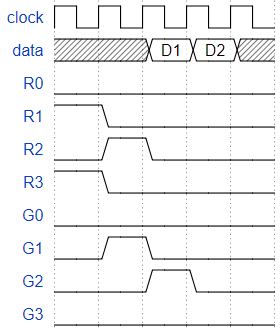
\includegraphics[width=3in]{problem3b.png}
        \end{center}
\end{figure}

\paragraph{b)}

The timing diagram for my design is shown above. The arbiter first grants the bus to device 1, then device 2.

\section*{Problem 4}

\paragraph{a)}

I will add another data memory unit in the \texttt{WB} stage. During the \texttt{sb} instruction in the \texttt{MEM} stage, the data memory
performs a read from the given address. Then in the \texttt{WB} stage, the read data will be concatenated with the lowest 8 bits of the register
that contains the data to be stored. There are four ways to perform this concatenation based on the lowest two bits of the store address, so a multiplexer
will be used to choose which location to place the byte. Then the additional data memory unit is used to store the concatenated data in the store address.

\begin{figure}[!ht]
        \begin{center}
                \hspace*{-4cm}
                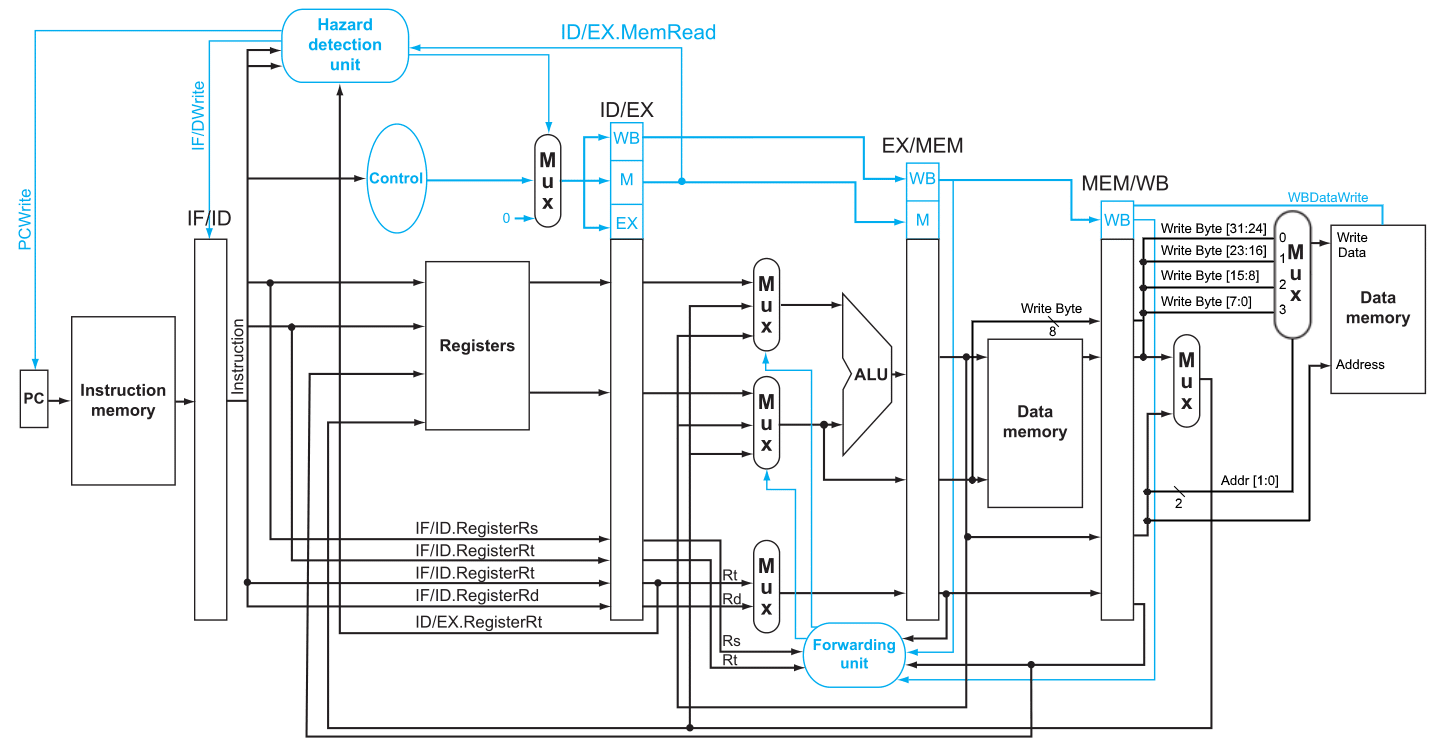
\includegraphics[width=6.5in]{problem4b.png}
                \hspace*{-4cm}
        \end{center}
\end{figure}

\paragraph{b)}

The following figure shows my modifications. Note that I do not include forwarding between the \texttt{WB} and \texttt{MEM} stages to correct for any data dependencies
between a \texttt{lw} or \texttt{sw} that follows a \texttt{sb} instruction. To implement forwarding, I would have to check if the target address of the \texttt{lw} or
\texttt{sw} is the same as the \texttt{sb}, and either replace the read contents for \texttt{lw} or have the write for \texttt{sw} override the write for \texttt{sb}.

Note that the label \texttt{Write Byte [31:24]} is a 32-bit signal that indicates the read data with bits 24 to 31 replaced by the 8 bit \texttt{Write Byte} signal, and
similarly for the other four inputs to the multiplexer.

\paragraph{c)}

A new control signal called \texttt{WBDataWrite} is needed, which controls the write in the WB stage.

\paragraph{d)}

The changes to the control unit are shown in the following table.
\begin{center}
       {\scriptsize
        \hspace*{-4cm}
        \begin{tabular}{c|c|c|c|c|c|c|c|c|c|c}
                Instruction & \texttt{RegDst} & \texttt{ALUOp1} & \texttt{ALUOp0} & \texttt{ALUSrc} & \texttt{Branch} & \texttt{MemRead}
                & \texttt{MemWrite} & \texttt{RegWrite} & \texttt{MemtoReg} & \texttt{WBDataWrite}\\
                \hline
                R-Format & 1 & 1 & 0 & 0 & 0 & 0 & 0 & 1 & 0 & 0\\
                \texttt{lw} & 0 & 0 & 0 & 1 & 0 & 1 & 0 & 1 & 1 & 0\\
                \texttt{sw} & x & 0 & 0 & 1 & 0 & 0 & 1 & 0 & x & 0\\
                \texttt{sb} & x & 0 & 0 & 1 & 0 & 1 & 0 & 0 & x & 1\\
                \texttt{beq} & x & 0 & 1 & 0 & 1 & 0 & 0 & 0 & x & 0
        \end{tabular}
        \hspace{-4cm}
        }
\end{center}

\section*{Problem 5}

Sequence A could be completed faster, as reads using DRAM only require a read-write cycle to ensure that the charge in the capacitors is refreshed,
while writes require a read-modify-write cycle to change the data in the specified address. When writing, we must read before modifying because we can only write
an entire row at once, so we must first know what the values stored in the row are. Then we change the specified bit, and write back. Thus writing has strictly more
operations to perform than reading, so reading can be completed faster.

\section*{Problem 6}

There are 32 instruction bits and 32 data bits that can be read every cycle, so this would require at least 8 of the given chips to supply the required 64 bits
of output. Thus the size of our memory would be \(2^{27}\) bits, or \(128\) Mibit.

\end{document}